% Mirror: https://github.com/SIGma-UIUC/presentation-format
% --------------------------------------------------------------------
% This is a simple Beamer document that uses beamerthemesigma.sty
% Reading the comments should help you create a presentation even if
% you've never used Beamer before.
% --------------------------------------------------------------------

% Set our document class to Beamer
\documentclass[aspectratio=169]{beamer}

% Some packages for nice font encodings in the final PDF
\usepackage[utf8]{inputenc}
\usepackage[T1]{fontenc}

% From Jeff E
\usepackage{algo}

% Some more macros
\usepackage{sigmastyle}

% Citations
\usepackage{cite}

% To insert images
\usepackage{graphicx}

% Useful packages from the AMS
\usepackage{amsmath,amssymb,amsthm}

\usepackage{soul}

% Package for code highlighting
\usepackage{minted}
\setminted{linenos=true, breaklines=true, breakanywhere=true, style=default}
\usemintedstyle{monokai}

% Set a title
\title{The PACE 2023 Challenge: Twin-Width}

% Set a subtitle if you desire
\subtitle{}

% Whoever worked on the presentation:
\author{Anakin}

% Date looks ugly, so leave blank
\date{}

% An institute name, if you're so inclined
% \institute{University of Illinois Urbana-Champaign}

% Use the SIGma theme for this Beamer presentation
\usetheme{sigma}
% --------------------------------------------------------------------

% Begin document
\begin{document}

% Beamer calls each slide a "frame", defined within the environment:
% \begin{frame}
%   <frame content here>
% \end{frame}

% This frame is just the title.
\begin{frame}
\titlepage
\end{frame}

% A frame with the table of contents.
% This frame's title is "Outline".
\begin{frame}{Outline}
  \tableofcontents
\end{frame}

% \begin{frame}{Updates!}
%   % Let's put some real content in this frame:
%   Weekly updates:
%   \begin{itemize}
%     \item SIGma is an excellent SIG.
%     \item I'm out of ideas for updates.
%   \end{itemize}
% \end{frame}

\section{What is Twin-width?}
\frame{\sectionpage}

\begin{frame}{What is Twin-width?}
    \begin{itemize}
        \item A large part of combinatorics is defining useful measures of the complexity of structures \pause
        \begin{itemize}
            \item How easy is it to construct the object? \pause
            \item Algorithmic Complexity \pause
            \item Efficient encodings \pause
            \item \textcolor{sigma@mainblue}{\emph{Decomposition}}
        \end{itemize}
    \end{itemize}
\end{frame}

\begin{frame}{Operations on Graphs: Disjoint Union}
    \begin{center}
        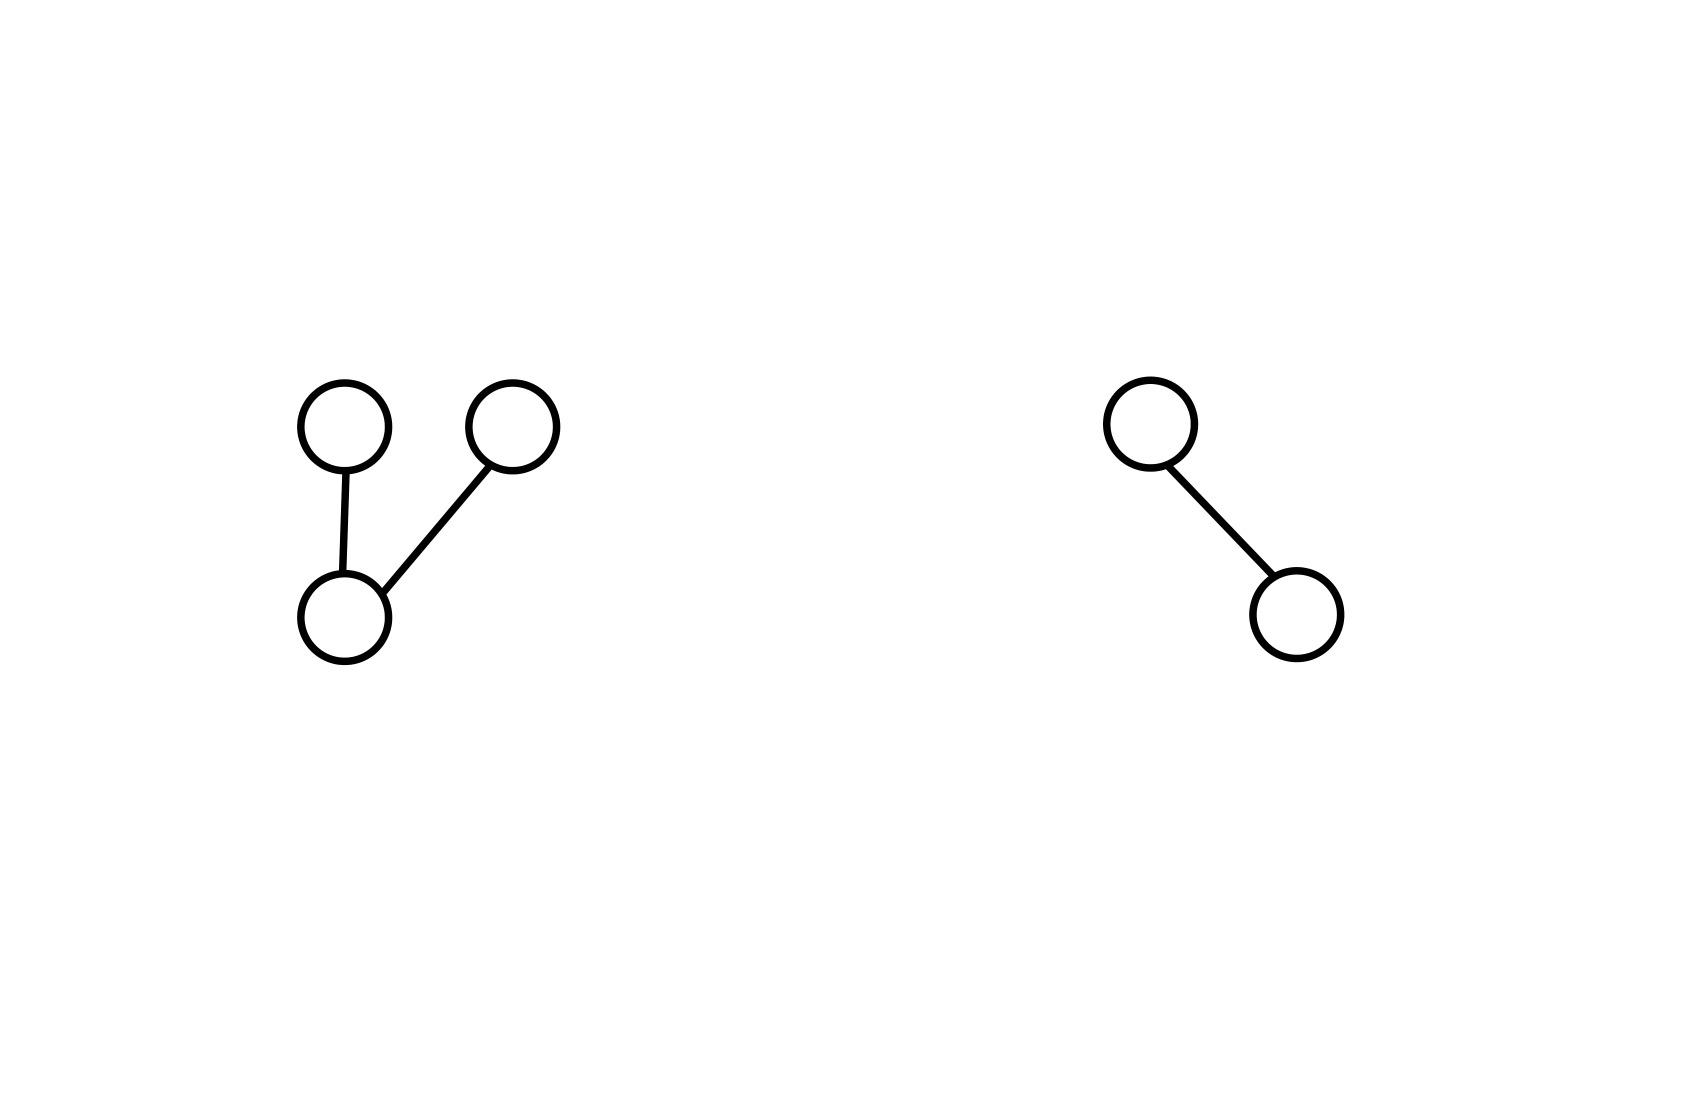
\includegraphics[width=1.0\textwidth]{images/output-13-0.jpg}
    \end{center}
\end{frame}

\begin{frame}{Operations on Graphs: Disjoint Union}
    \begin{center}
        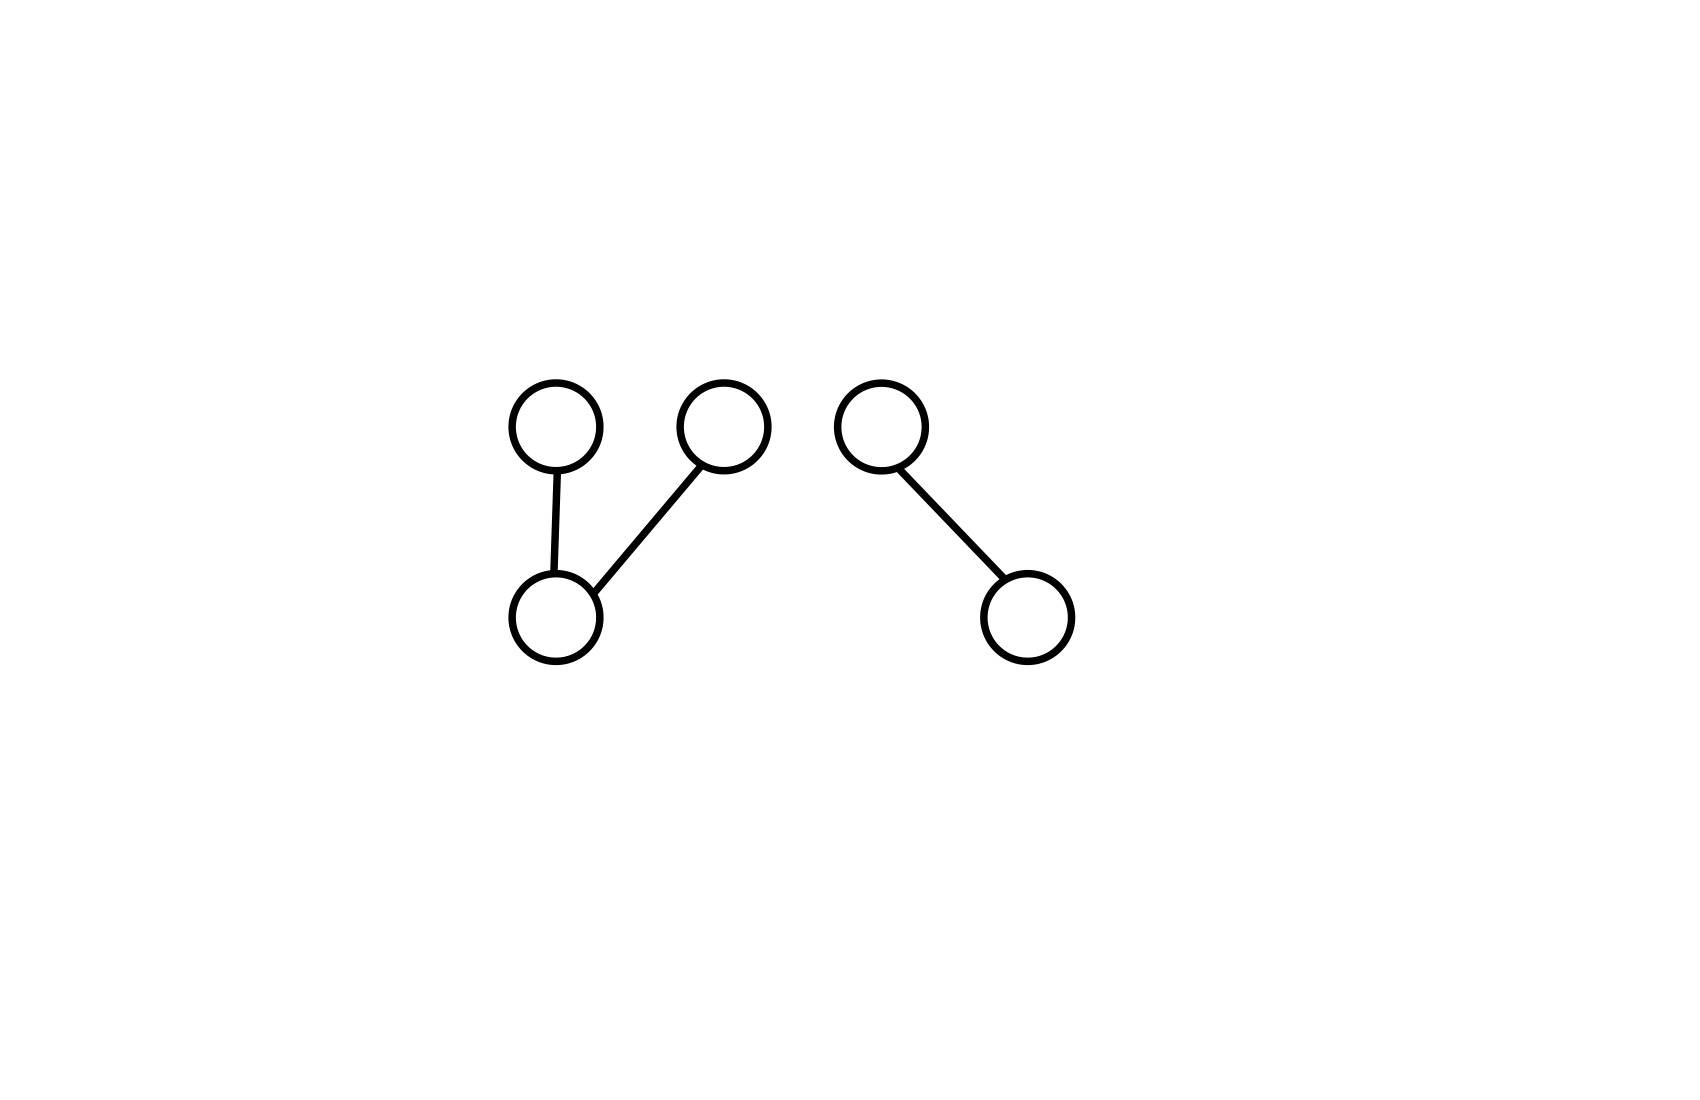
\includegraphics[width=1.0\textwidth]{images/output-14-0.jpg}
    \end{center}
\end{frame}

\begin{frame}{Operations on Graphs: Complement}
    \begin{center}
        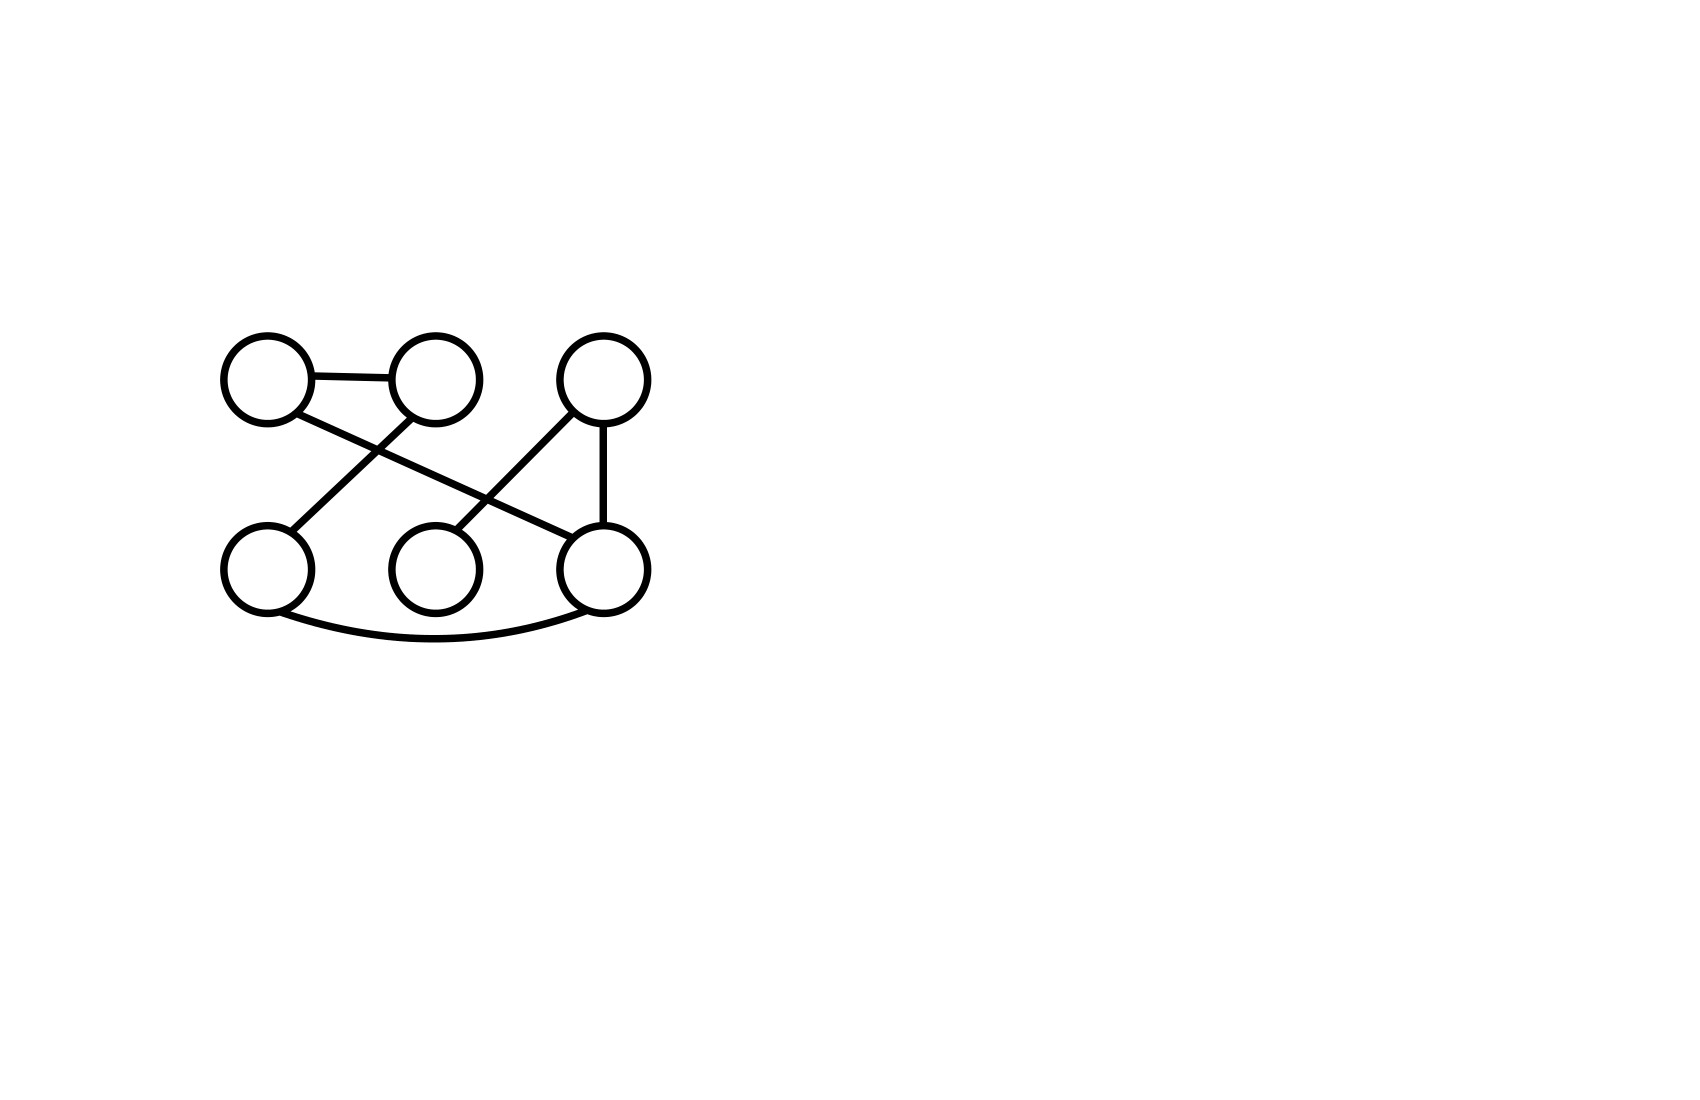
\includegraphics[width=1.0\textwidth]{images/output-15-0.jpg}
    \end{center}
\end{frame}

\begin{frame}{Operations on Graphs: Complement}
    \begin{center}
        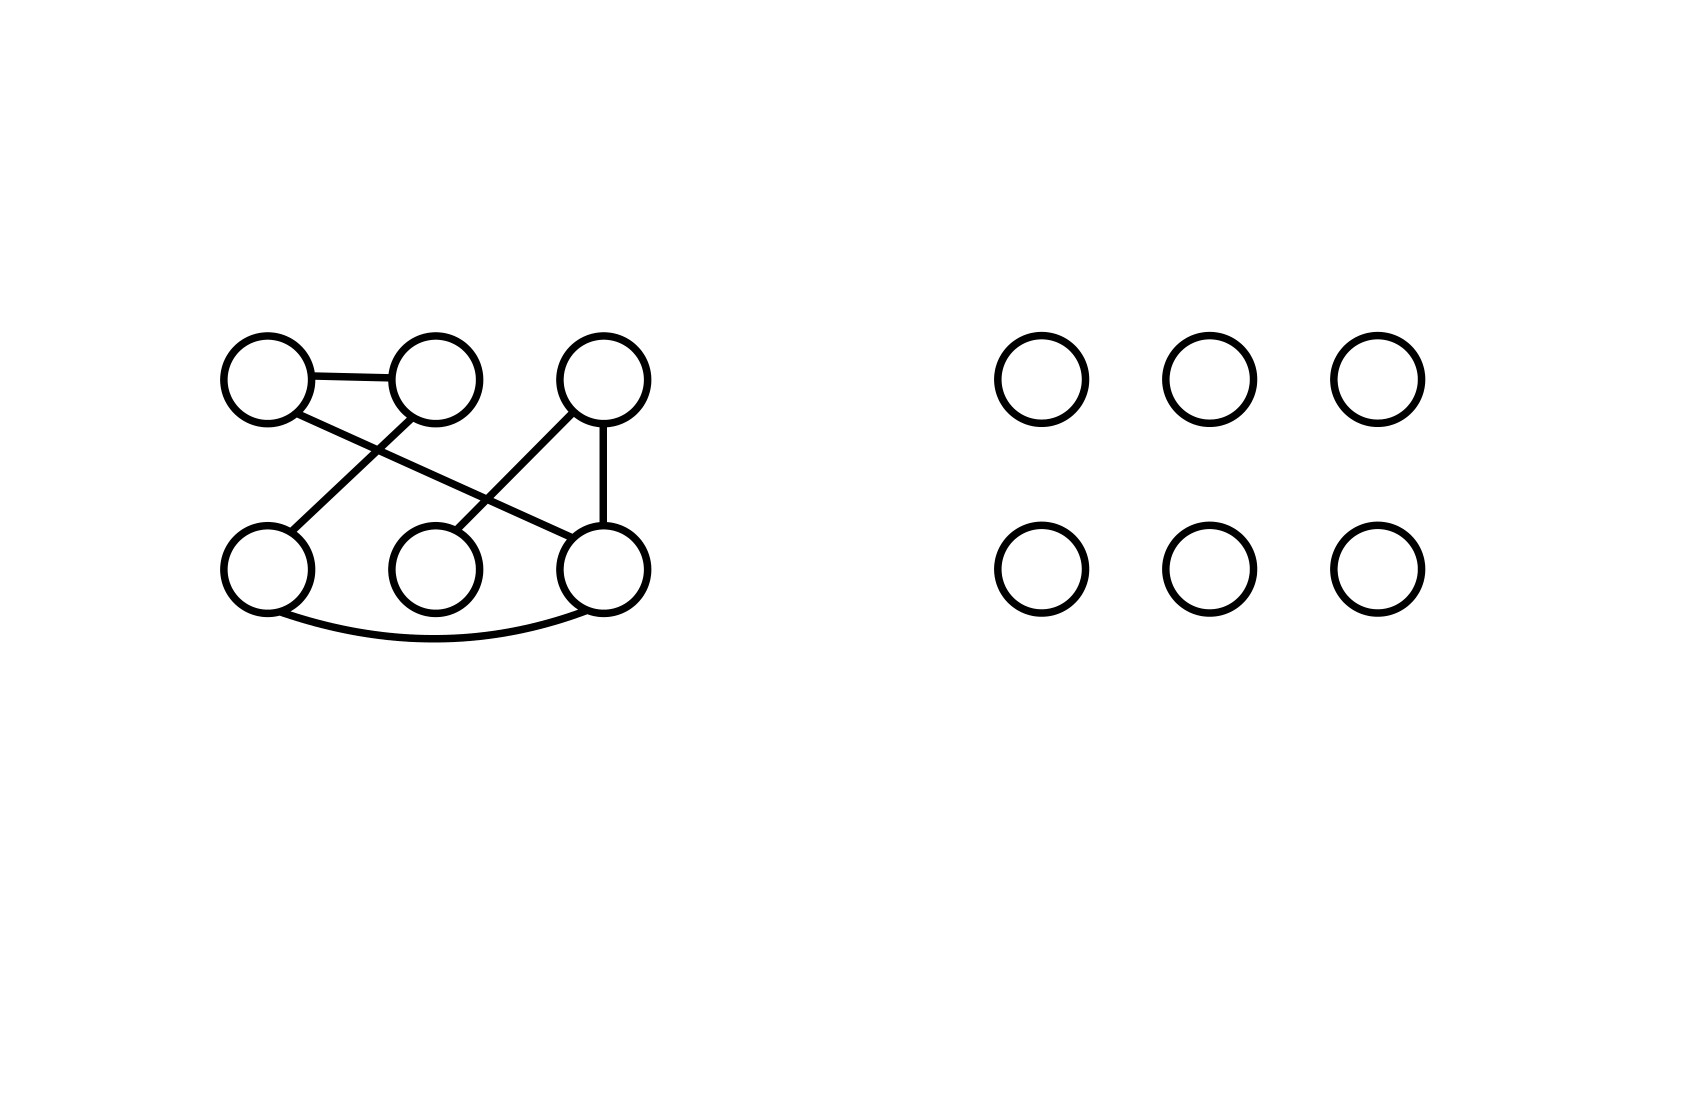
\includegraphics[width=1.0\textwidth]{images/output-16-0.jpg}
    \end{center}
\end{frame}

\begin{frame}{Operations on Graphs: Complement}
    \begin{center}
        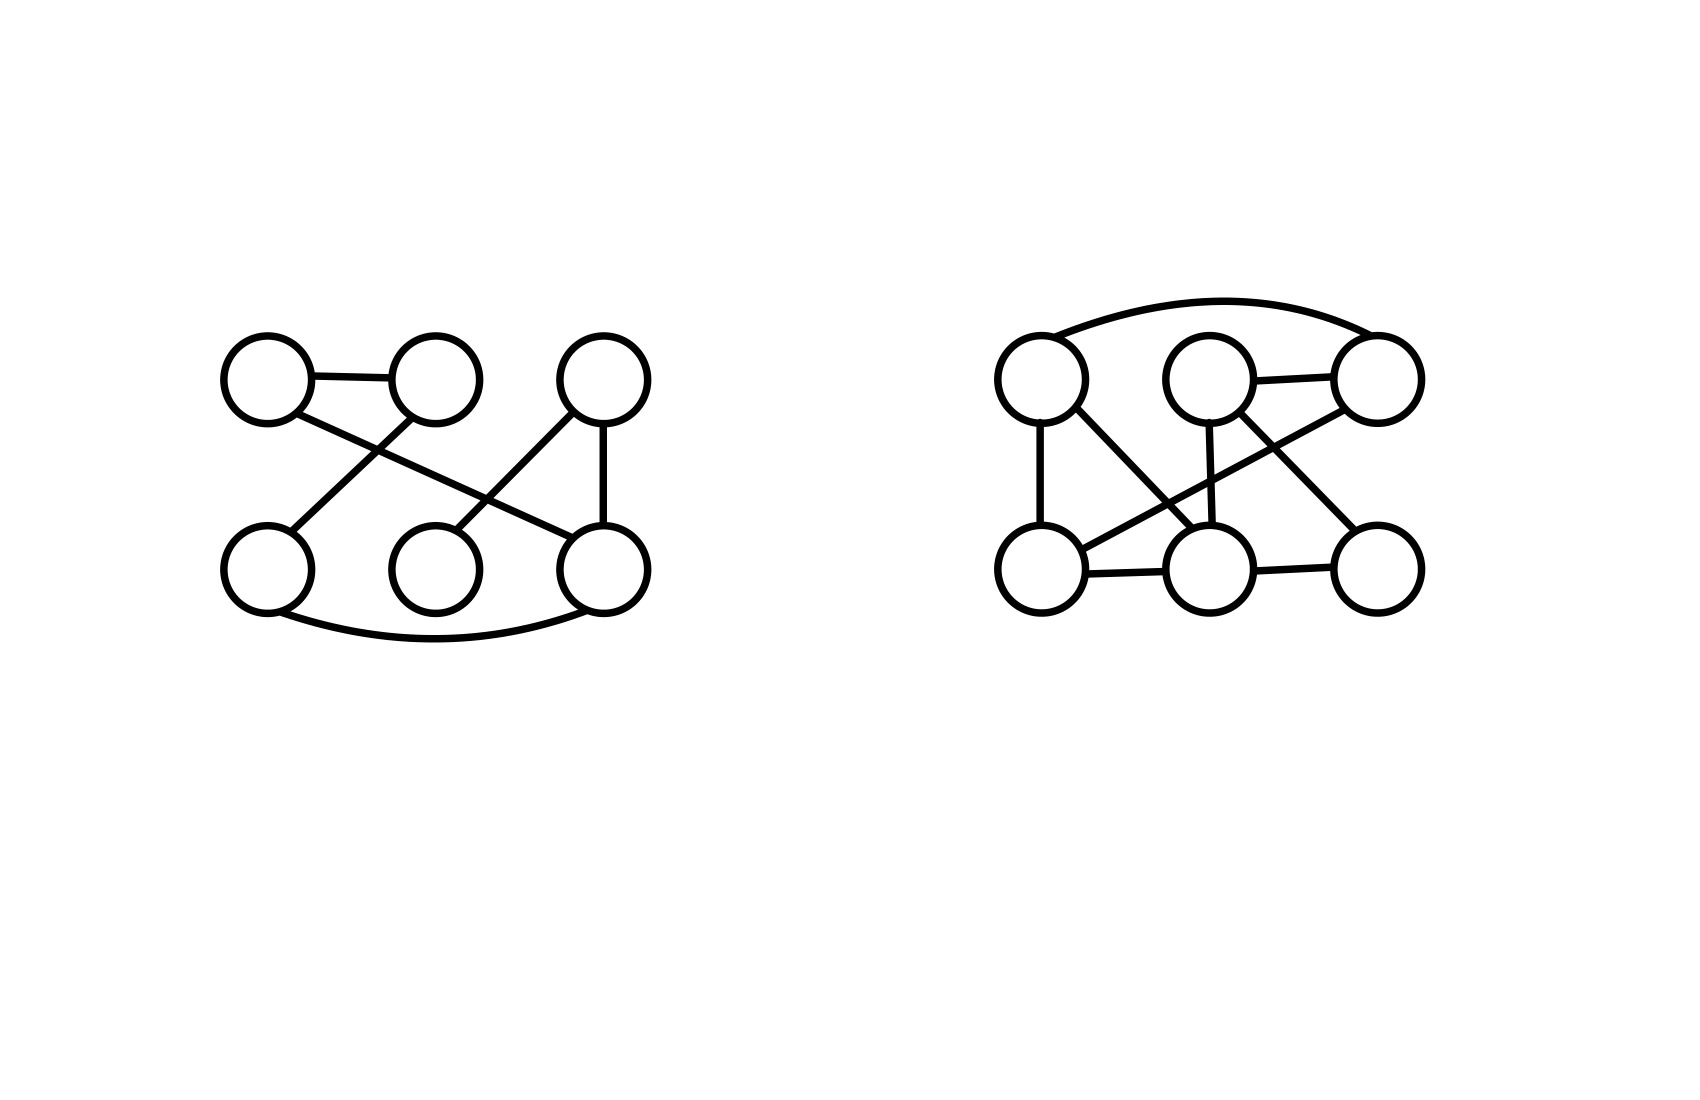
\includegraphics[width=1.0\textwidth]{images/output-17-0.jpg}
    \end{center}
\end{frame}


\begin{frame}{Cographs}
    We now construct the class of \textcolor{sigma@mainblue}{\emph{cographs}}\pause
    \begin{itemize}
        \item $K_1$ is a cograph
        \item The disjoint union of two cographs is also a cograph
        \item The complement of a cograph is a cograph
    \end{itemize}
\end{frame}

\begin{frame}{Relating Other Graphs to Cographs}
    \begin{itemize}
        \item This efficient way of constructing and decomposing these graphs is useful for many algorithms
        \begin{itemize}
            \item \underline{Example:} Finding the largest complete subgraph of a graph
        \end{itemize} \pause
        \item However, not every graph is a cograph 
        \item Can we generalize this by adding some sort of \textcolor{sigma@alertred}{\emph{error}} measure? \pause
        \item This is called \textcolor{sigma@mainblue}{\emph{twin-width}} \cite{Twin-width-I}
    \end{itemize}
\end{frame}

\begin{frame}{Contractions}
    \begin{itemize}
        \item Throughout this presentation, $G = (V, E)$ will be a connected undirected graph \pause
        \item Before we can talk about twin-width, we first talk about \textcolor{sigma@mainblue}{\emph{contractions}} of a graph \pause
        \begin{itemize}
            \item Our edges in $E$ will have a color associated with them: black or \textcolor{sigma@alertred}{red}.
            \begin{itemize}
                \item The red edges will be our \textcolor{sigma@alertred}{\emph{error}} that we want
            \end{itemize}
            \item Vertices are black neighbors if linked by a black edge, and red neighbors if linked by a red edge
        \end{itemize}
    \end{itemize}
\end{frame}

\begin{frame}{Contractions by picture}
    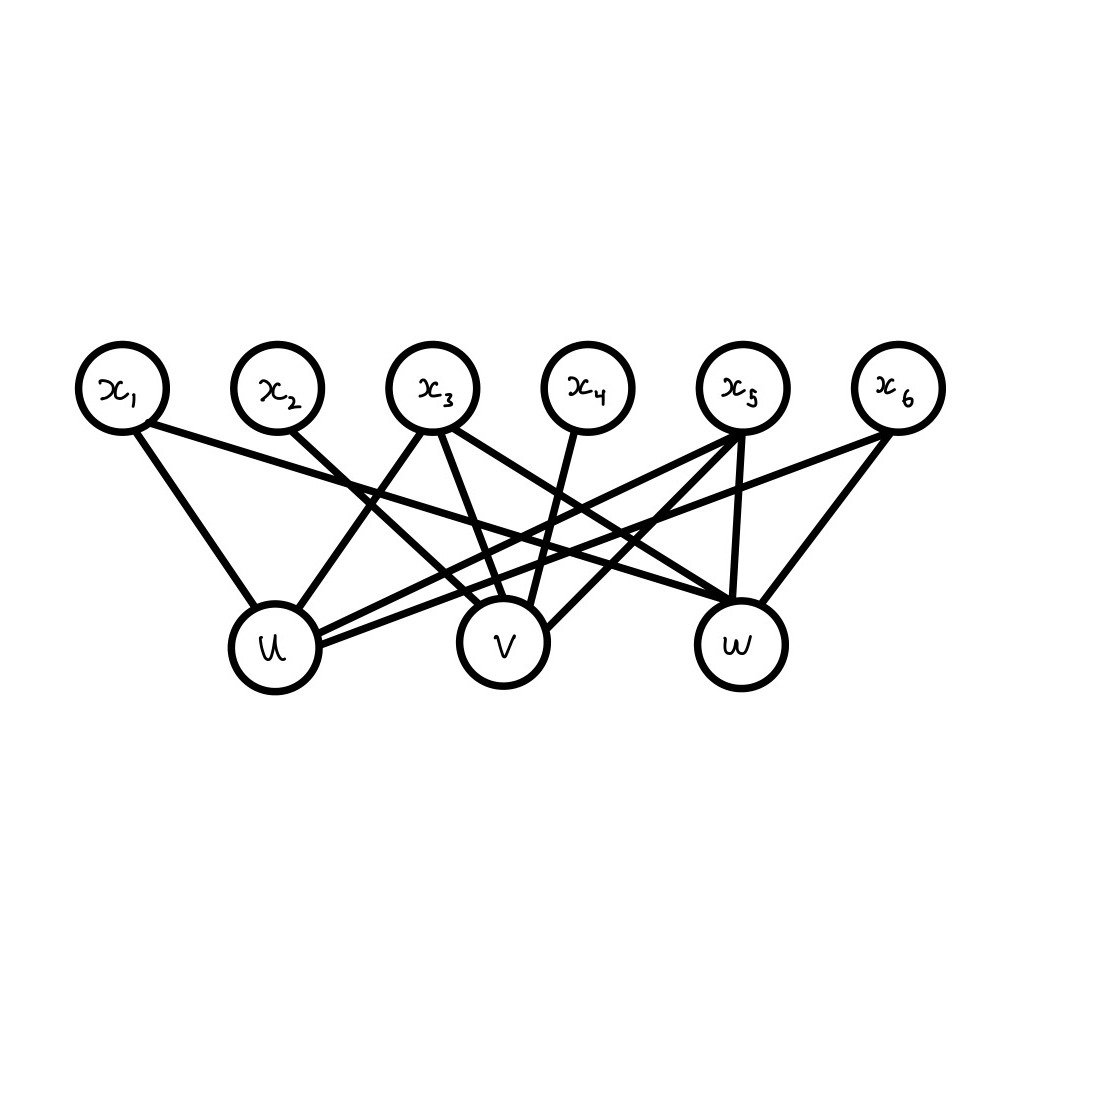
\includegraphics[width=0.5\textwidth]{images/cropped-01.jpg}%
    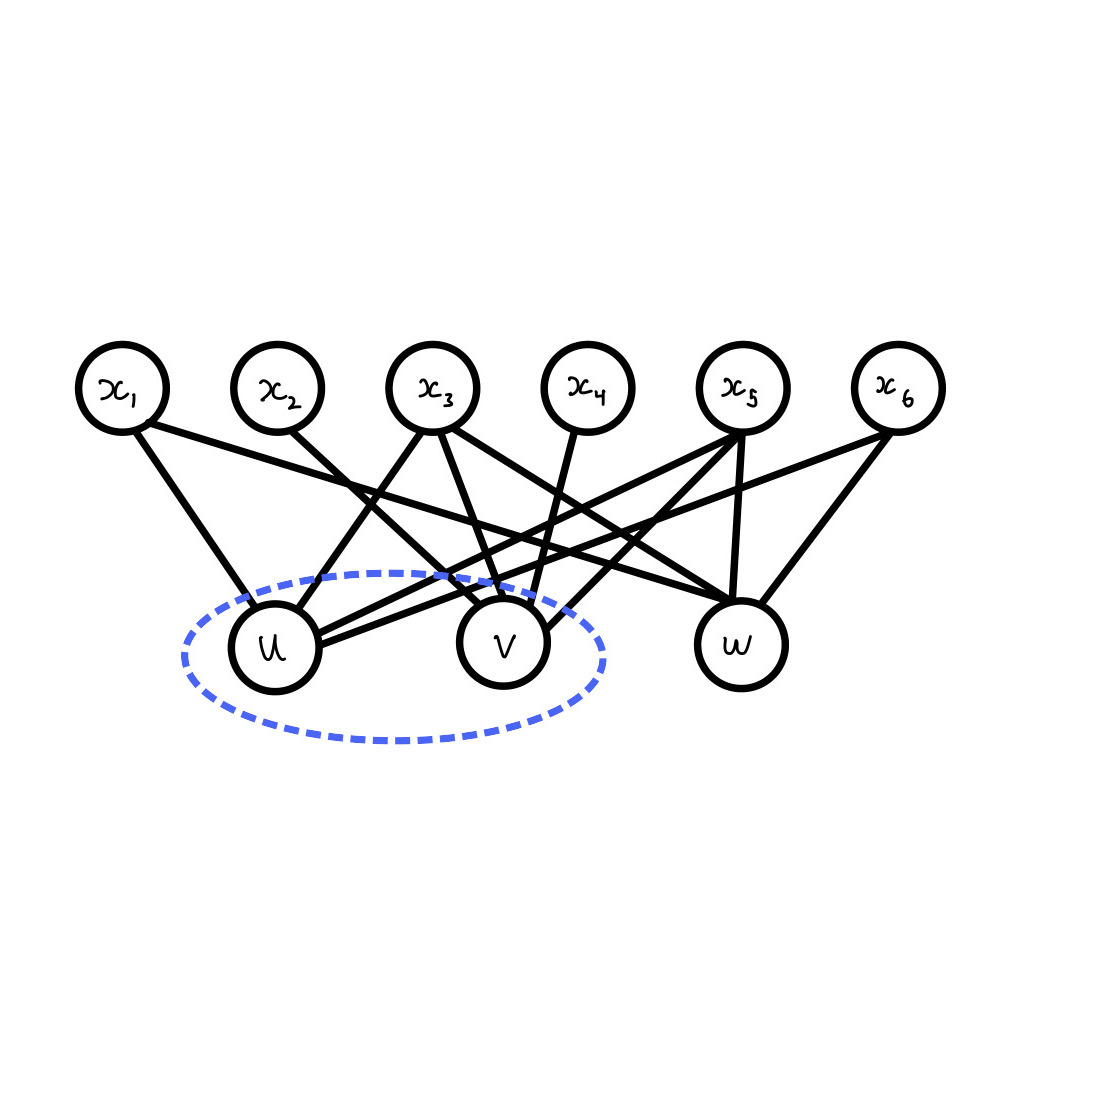
\includegraphics[width=0.5\textwidth]{images/cropped-02.jpg}
\end{frame}

\begin{frame}{Contractions by picture}
    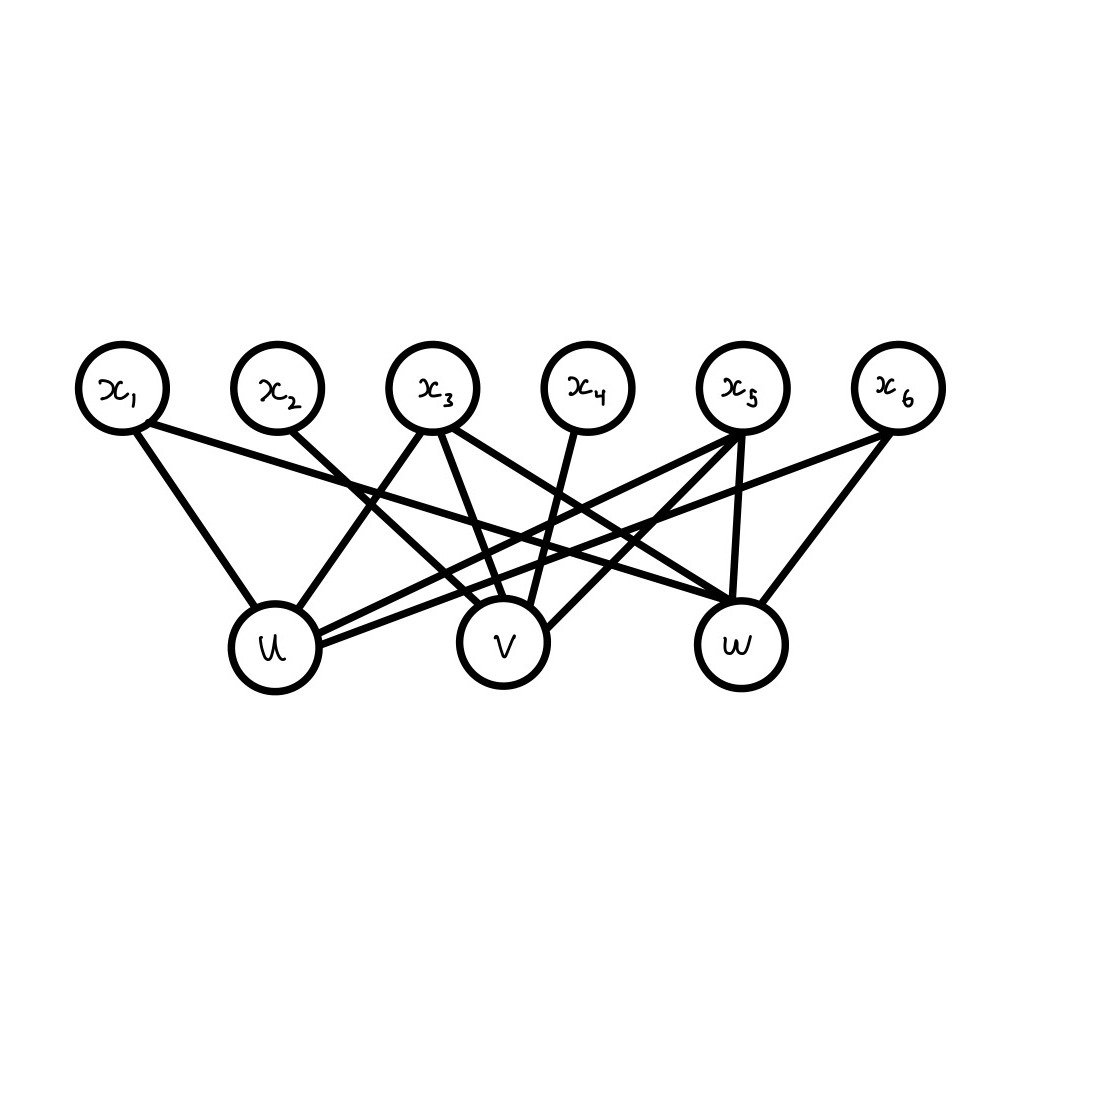
\includegraphics[width=0.5\textwidth]{images/cropped-01.jpg}%
    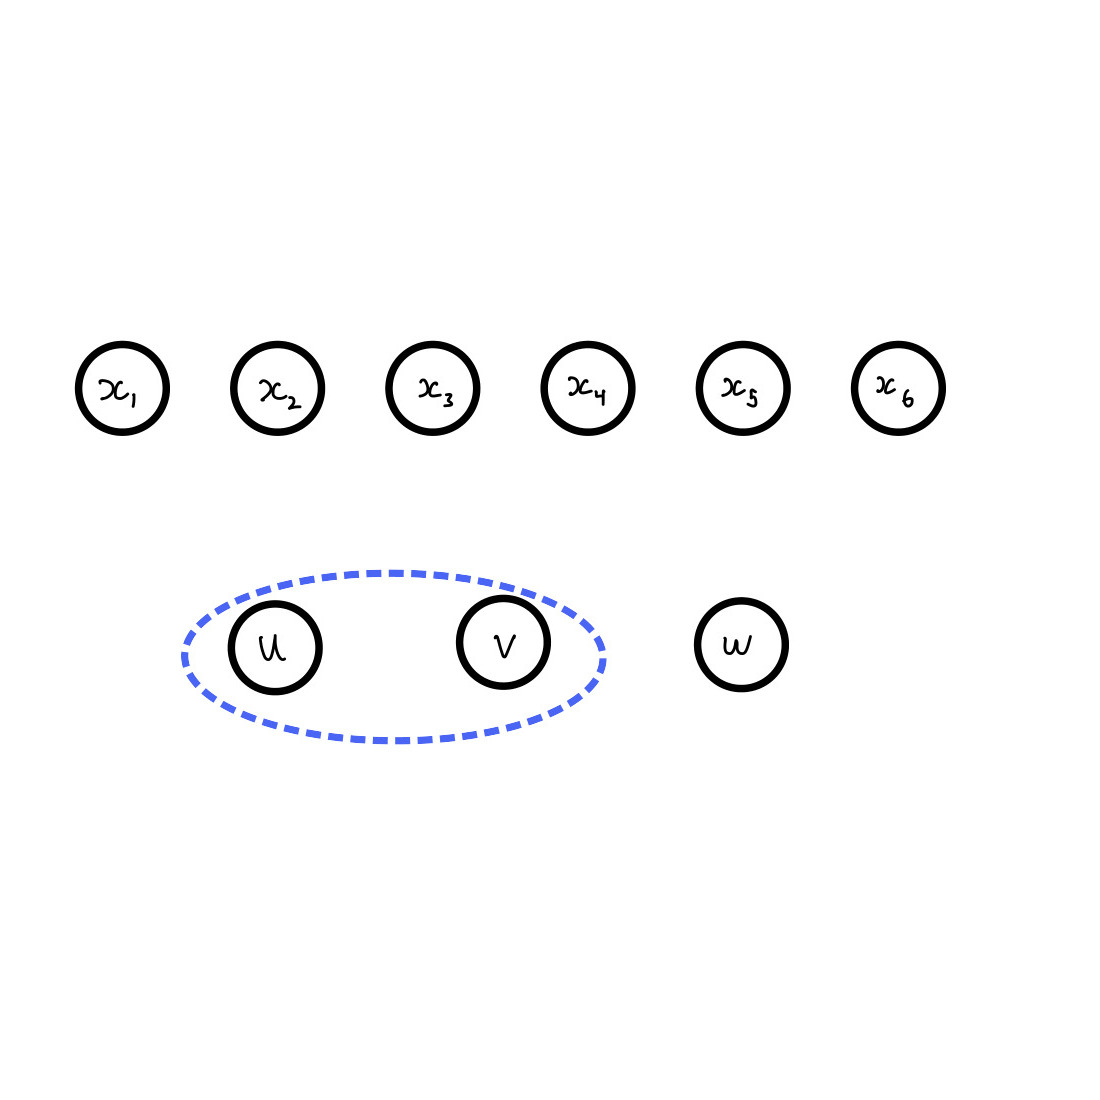
\includegraphics[width=0.5\textwidth]{images/cropped-03.jpg}
\end{frame}

\begin{frame}{Contractions by picture}
    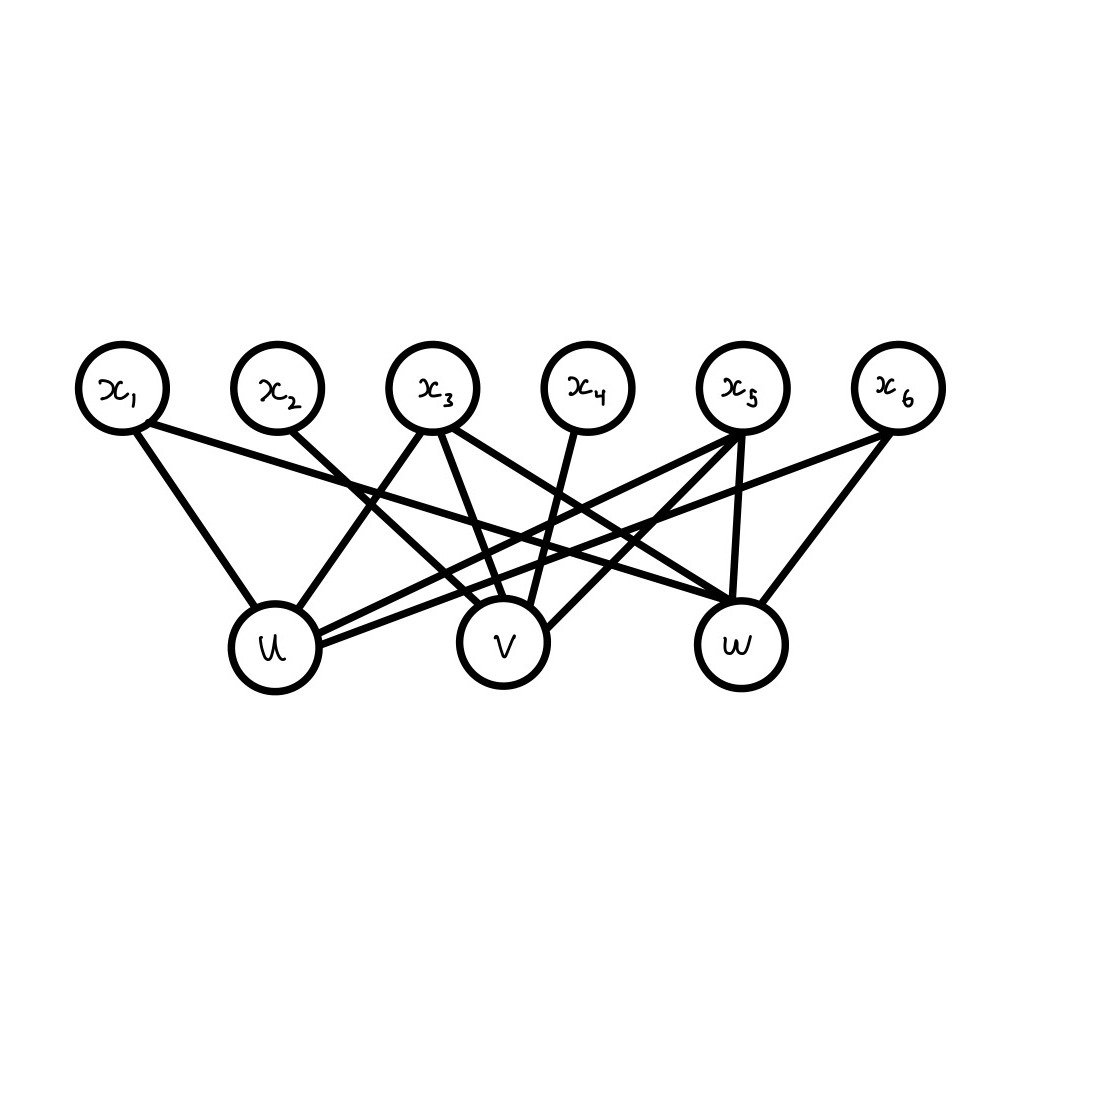
\includegraphics[width=0.5\textwidth]{images/cropped-01.jpg}%
    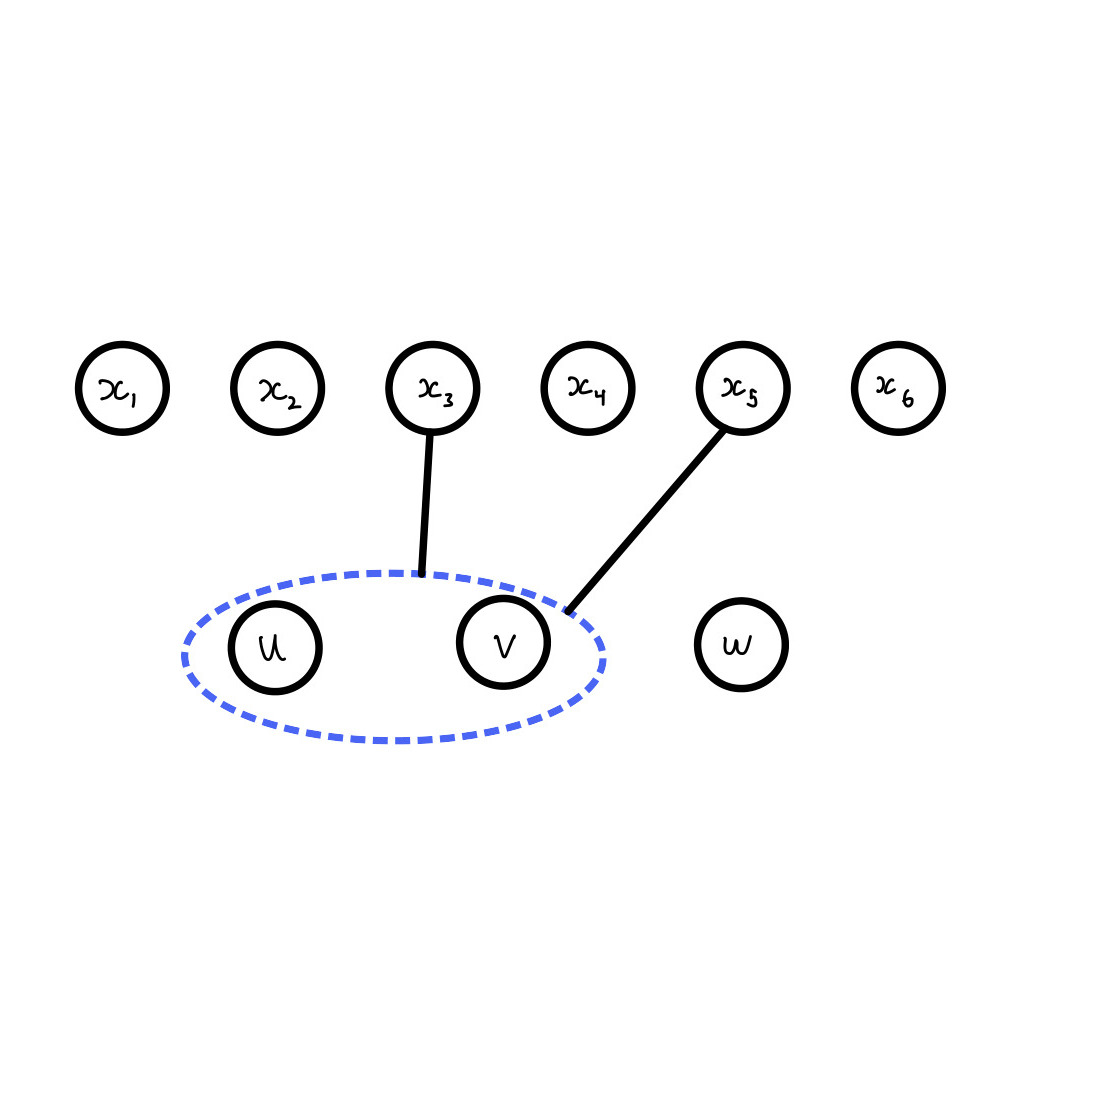
\includegraphics[width=0.5\textwidth]{images/cropped-04.jpg}
\end{frame}

\begin{frame}{Contractions by picture}
    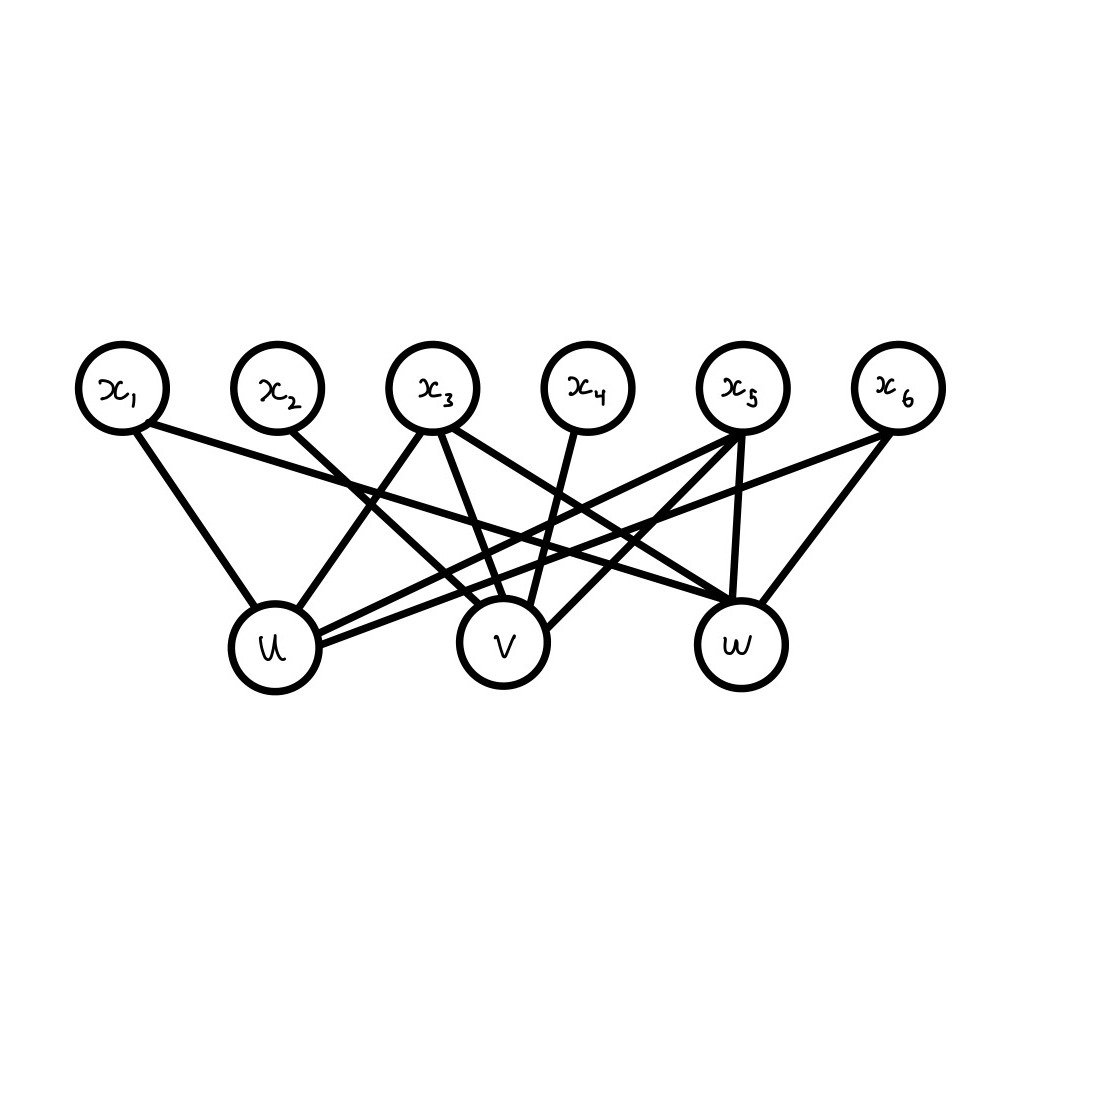
\includegraphics[width=0.5\textwidth]{images/cropped-01.jpg}%
    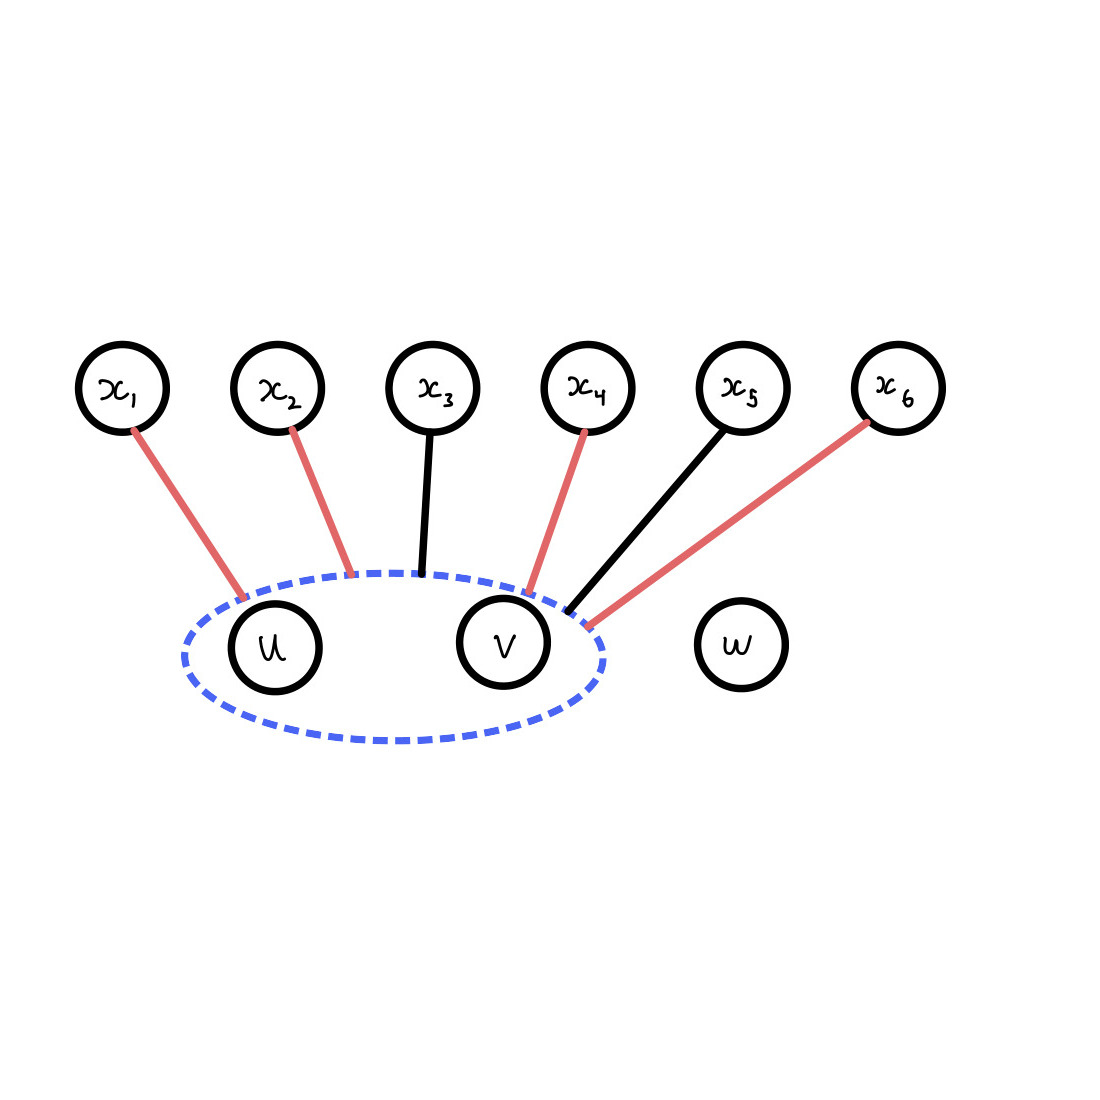
\includegraphics[width=0.5\textwidth]{images/cropped-05.jpg}
\end{frame}

\begin{frame}{Contractions by picture}
    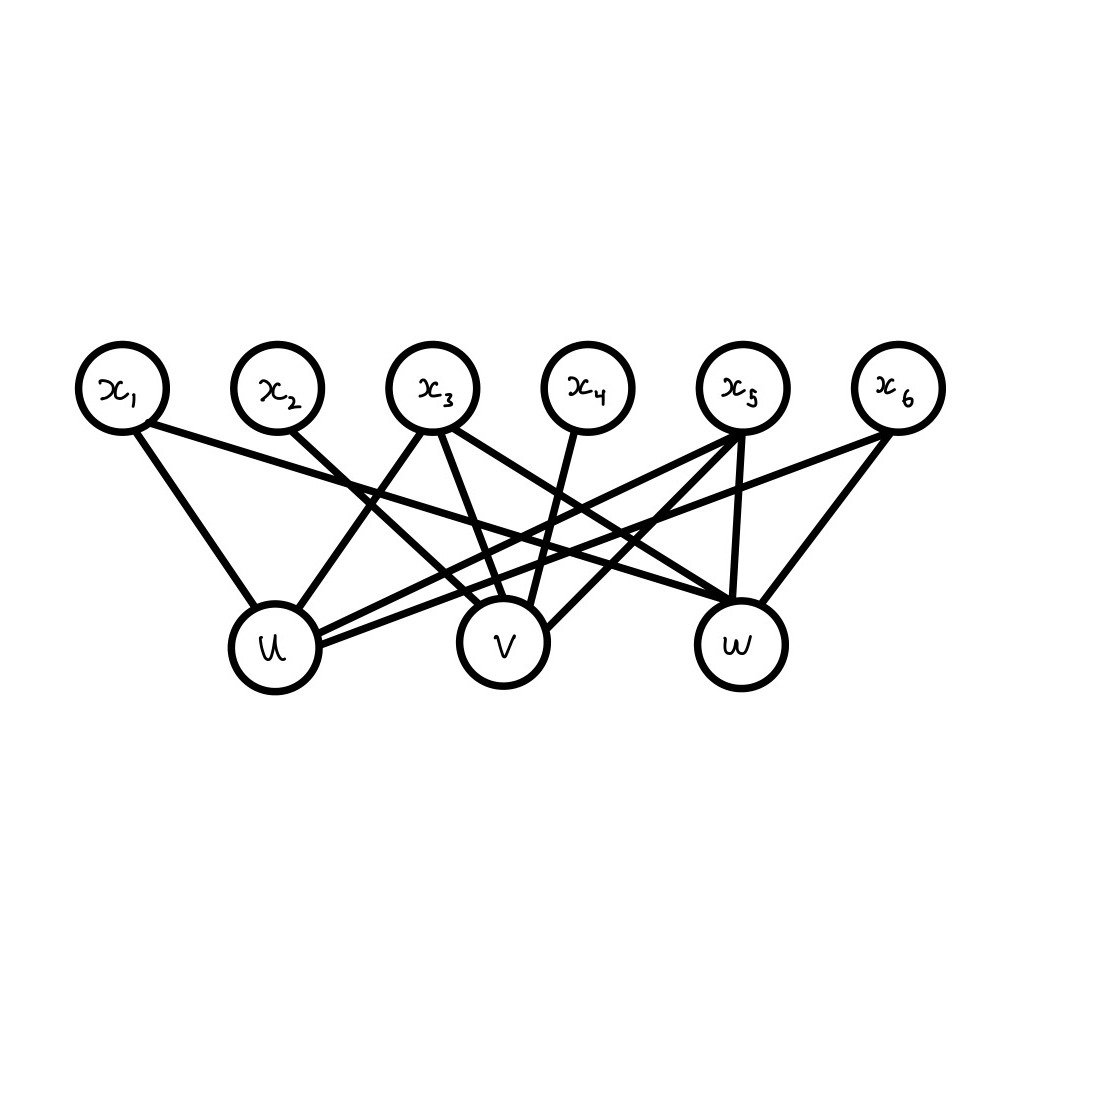
\includegraphics[width=0.5\textwidth]{images/cropped-01.jpg}%
    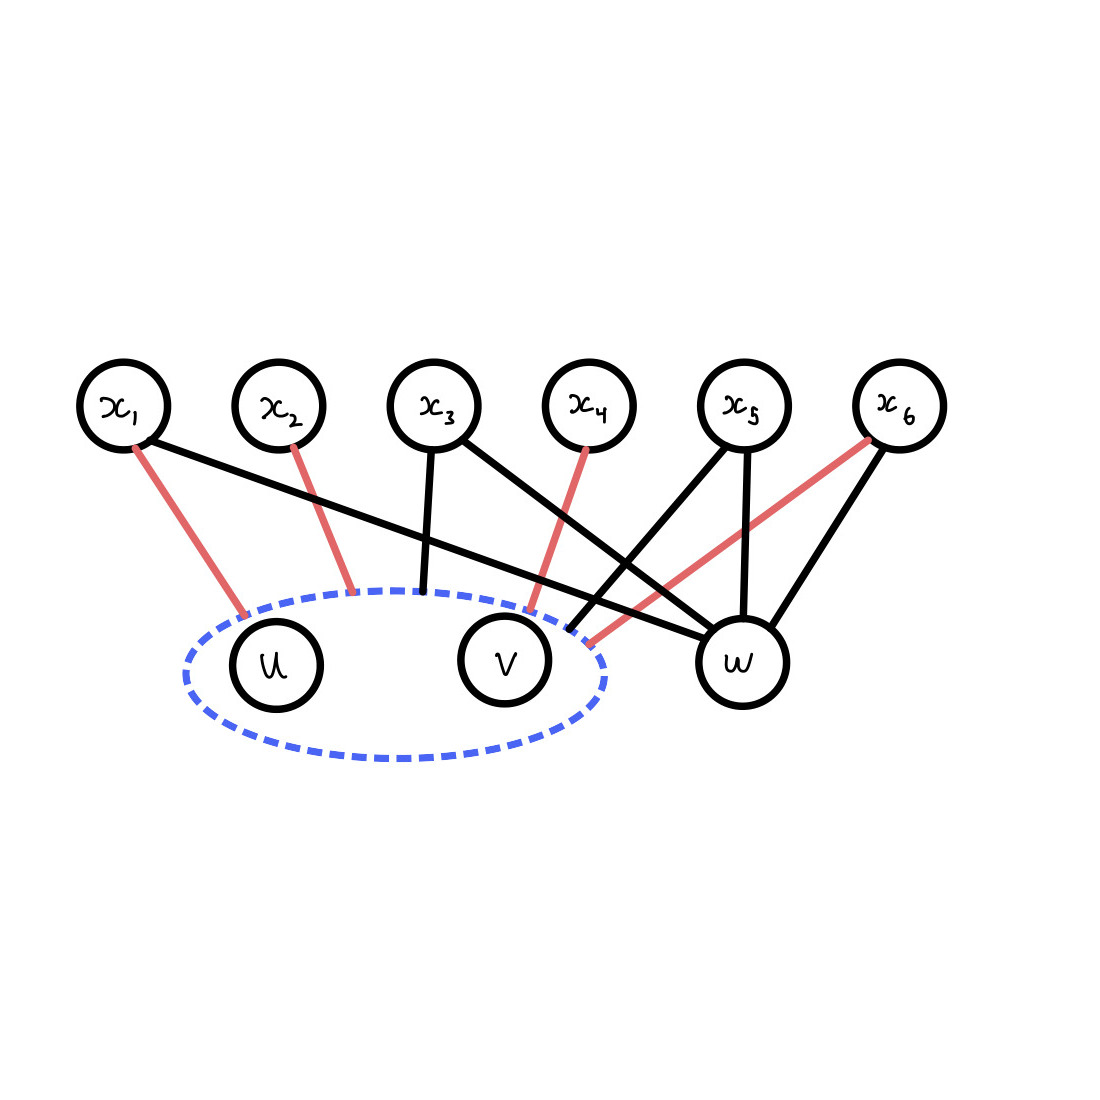
\includegraphics[width=0.5\textwidth]{images/cropped-06.jpg}
\end{frame}


\begin{frame}{Contractions by picture}
    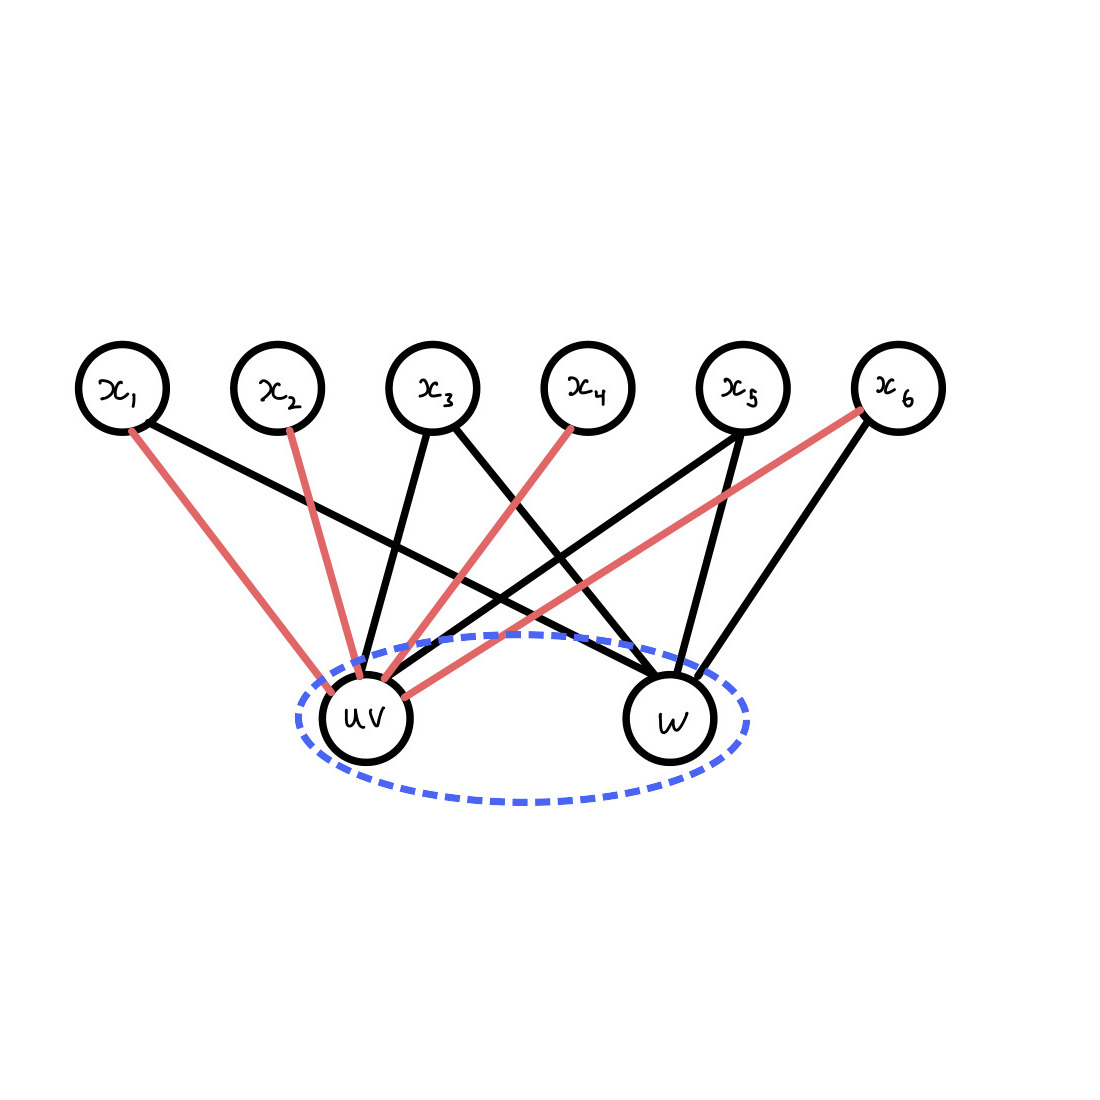
\includegraphics[width=0.5\textwidth]{images/cropped-08.jpg}%
    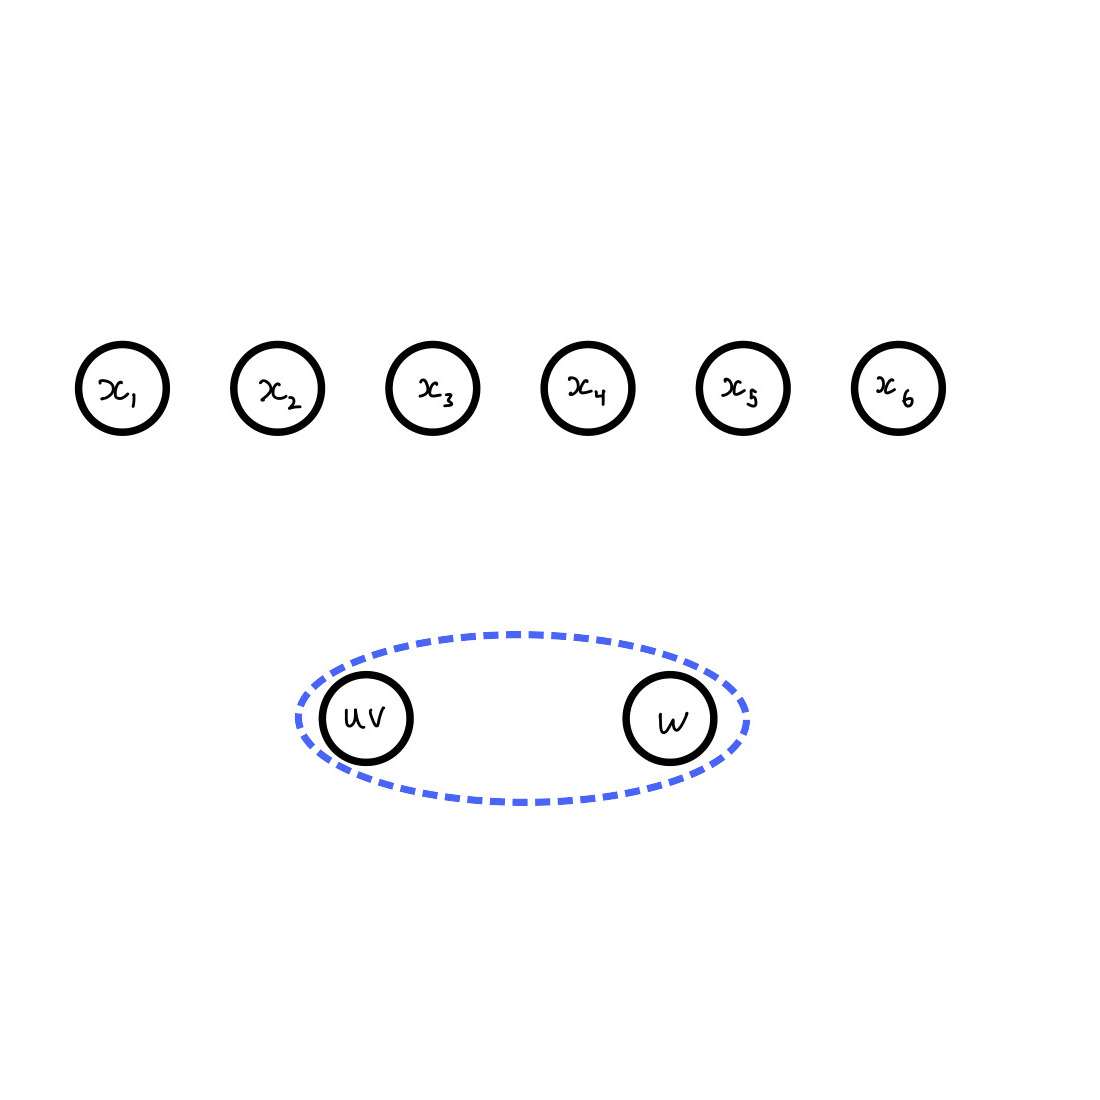
\includegraphics[width=0.5\textwidth]{images/cropped-09.jpg}
\end{frame}

\begin{frame}{Contractions by picture}
    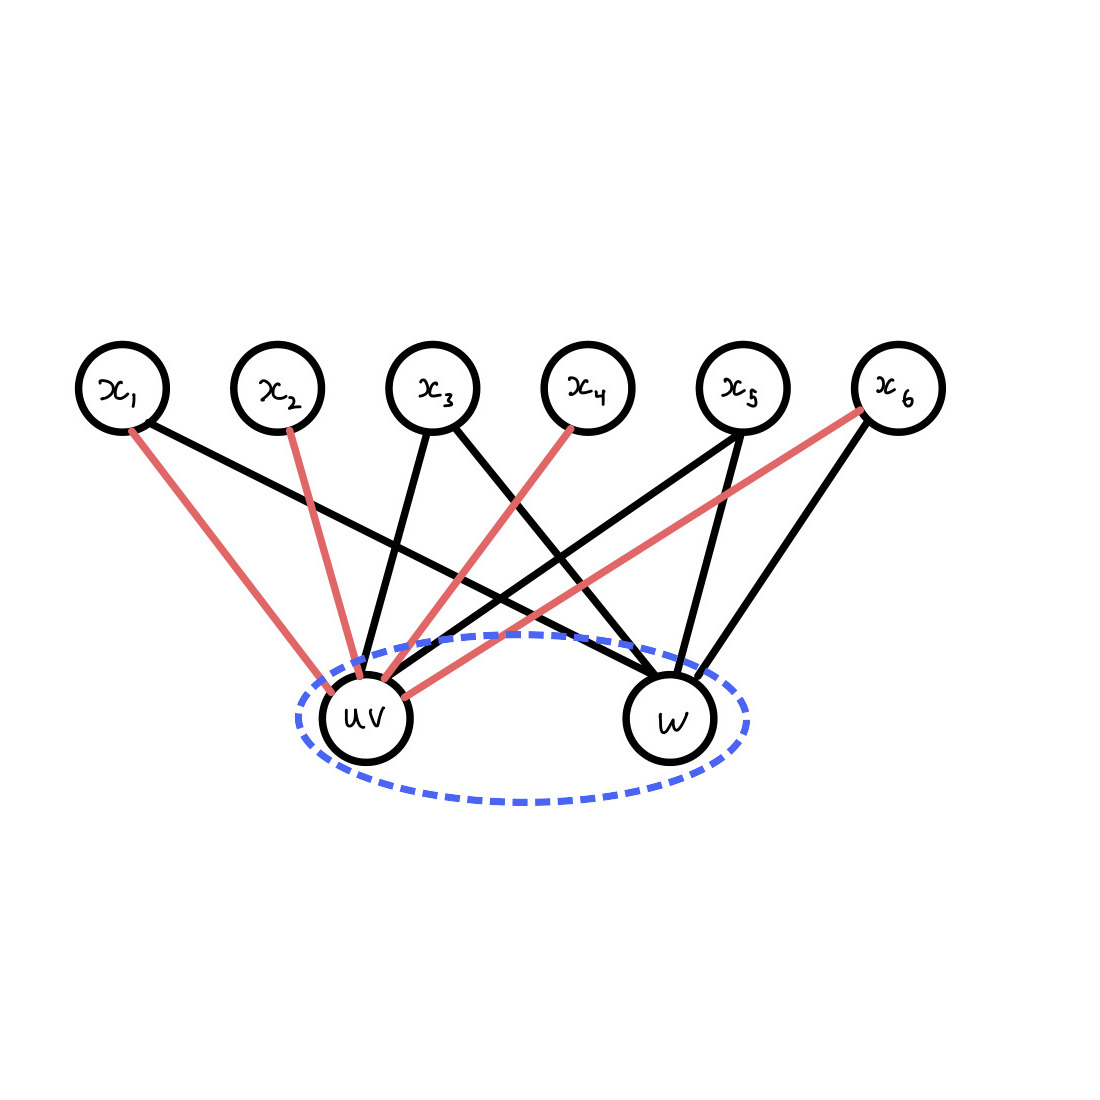
\includegraphics[width=0.5\textwidth]{images/cropped-08.jpg}%
    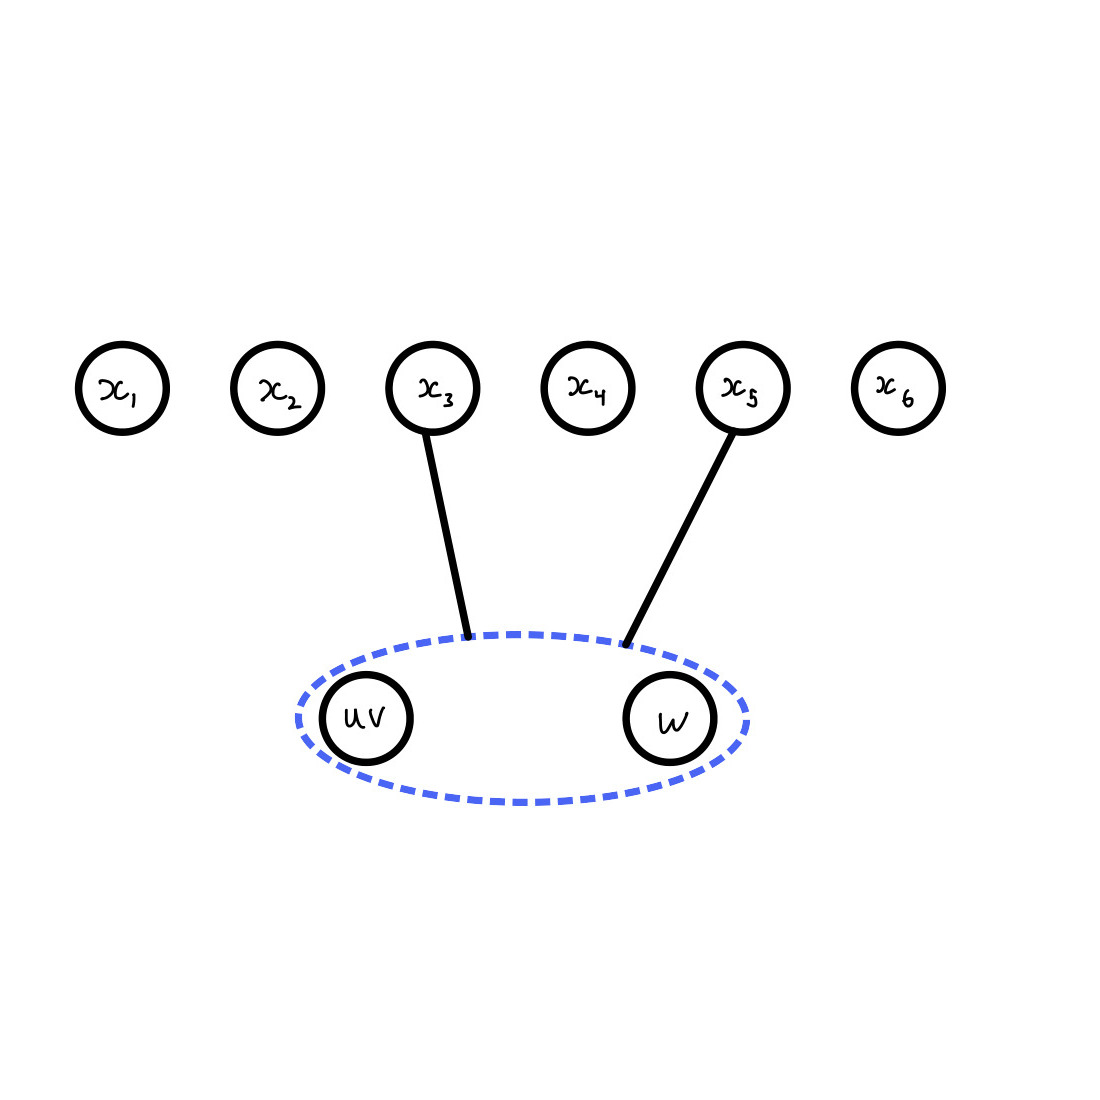
\includegraphics[width=0.5\textwidth]{images/cropped-10.jpg}
\end{frame}

\begin{frame}{Contractions by picture}
    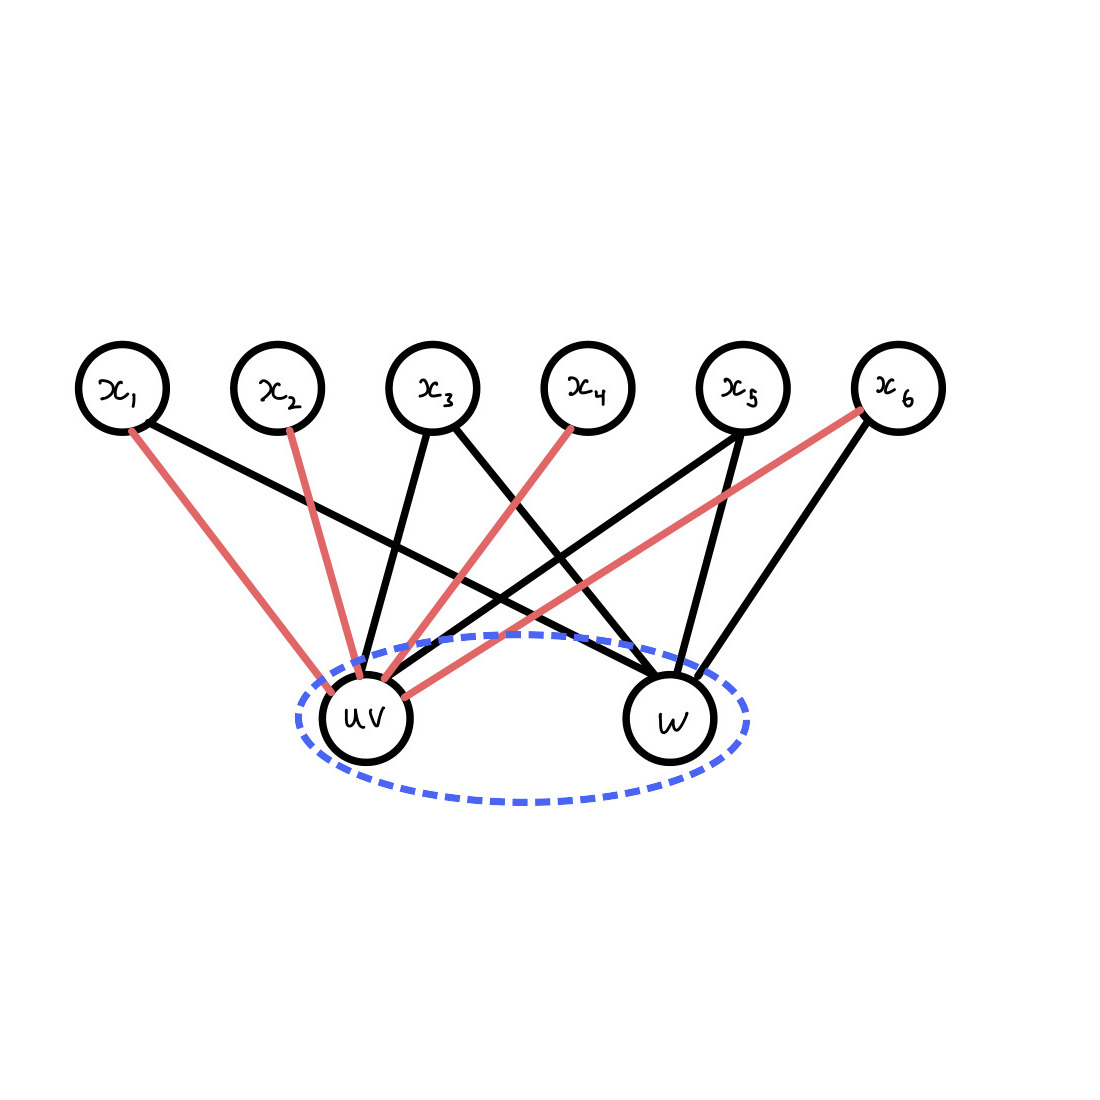
\includegraphics[width=0.5\textwidth]{images/cropped-08.jpg}%
    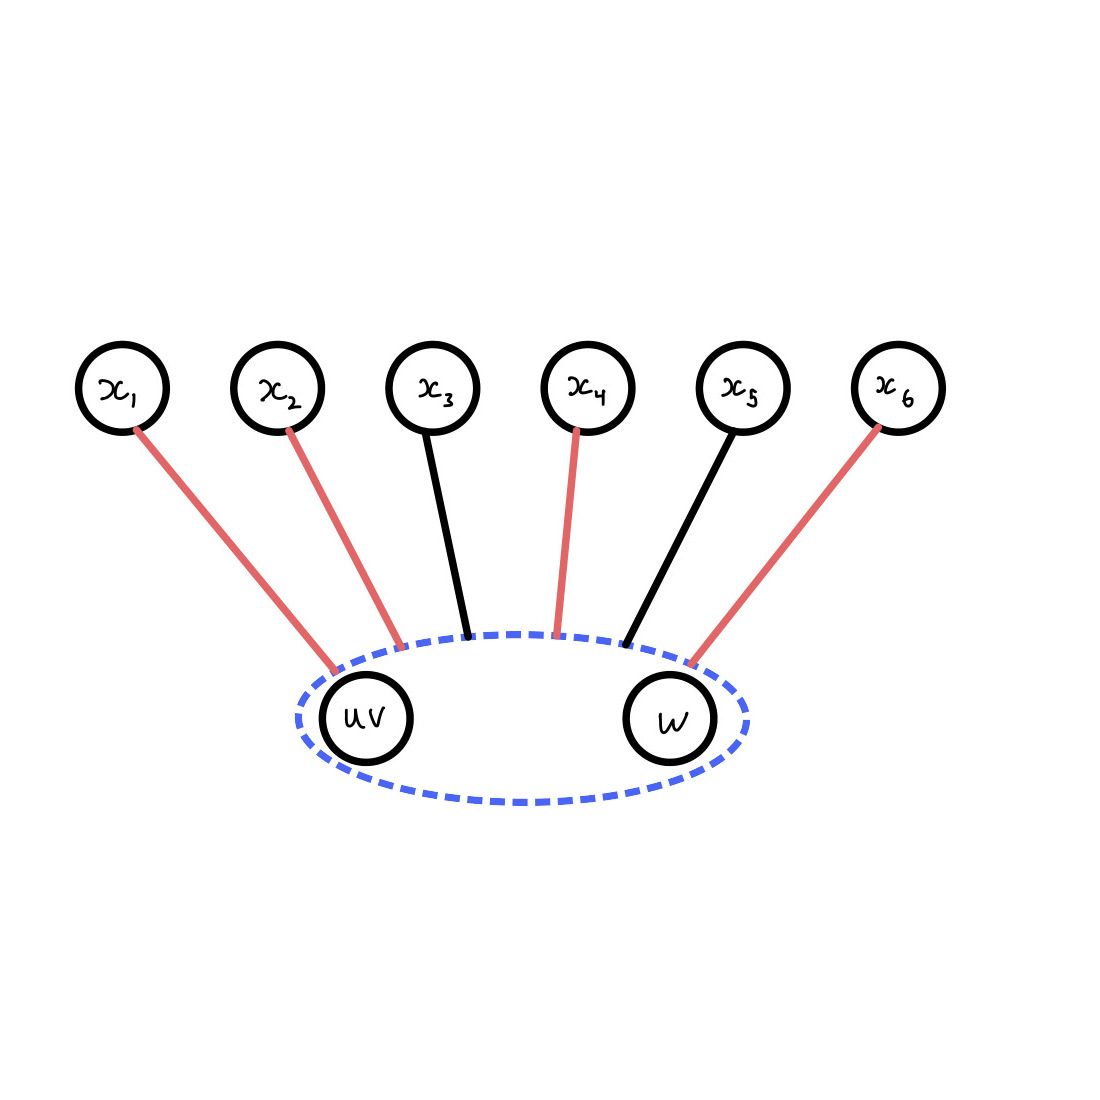
\includegraphics[width=0.5\textwidth]{images/cropped-11.jpg}
\end{frame}

\begin{frame}{Contractions by picture}
    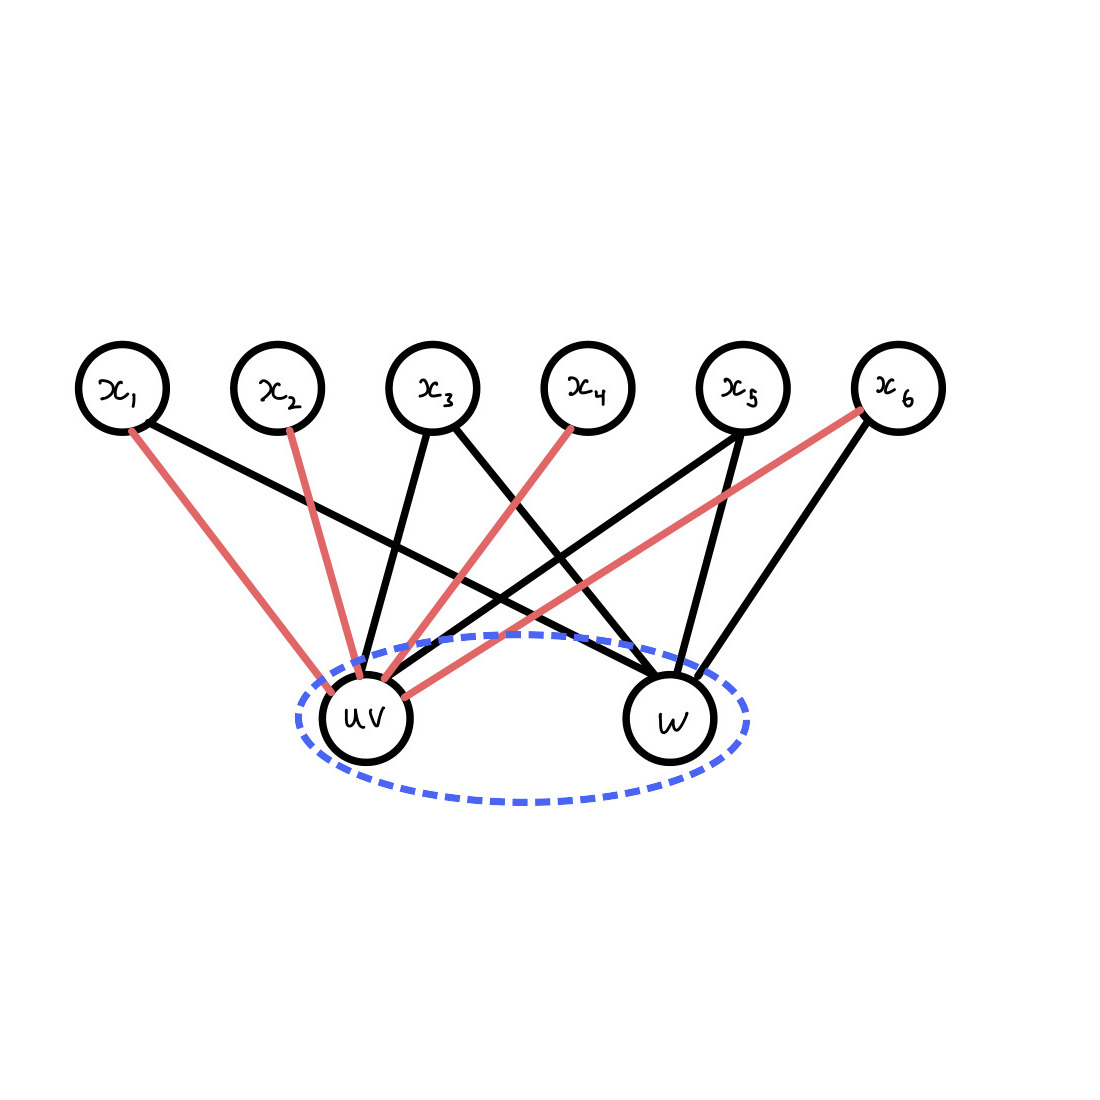
\includegraphics[width=0.5\textwidth]{images/cropped-08.jpg}%
    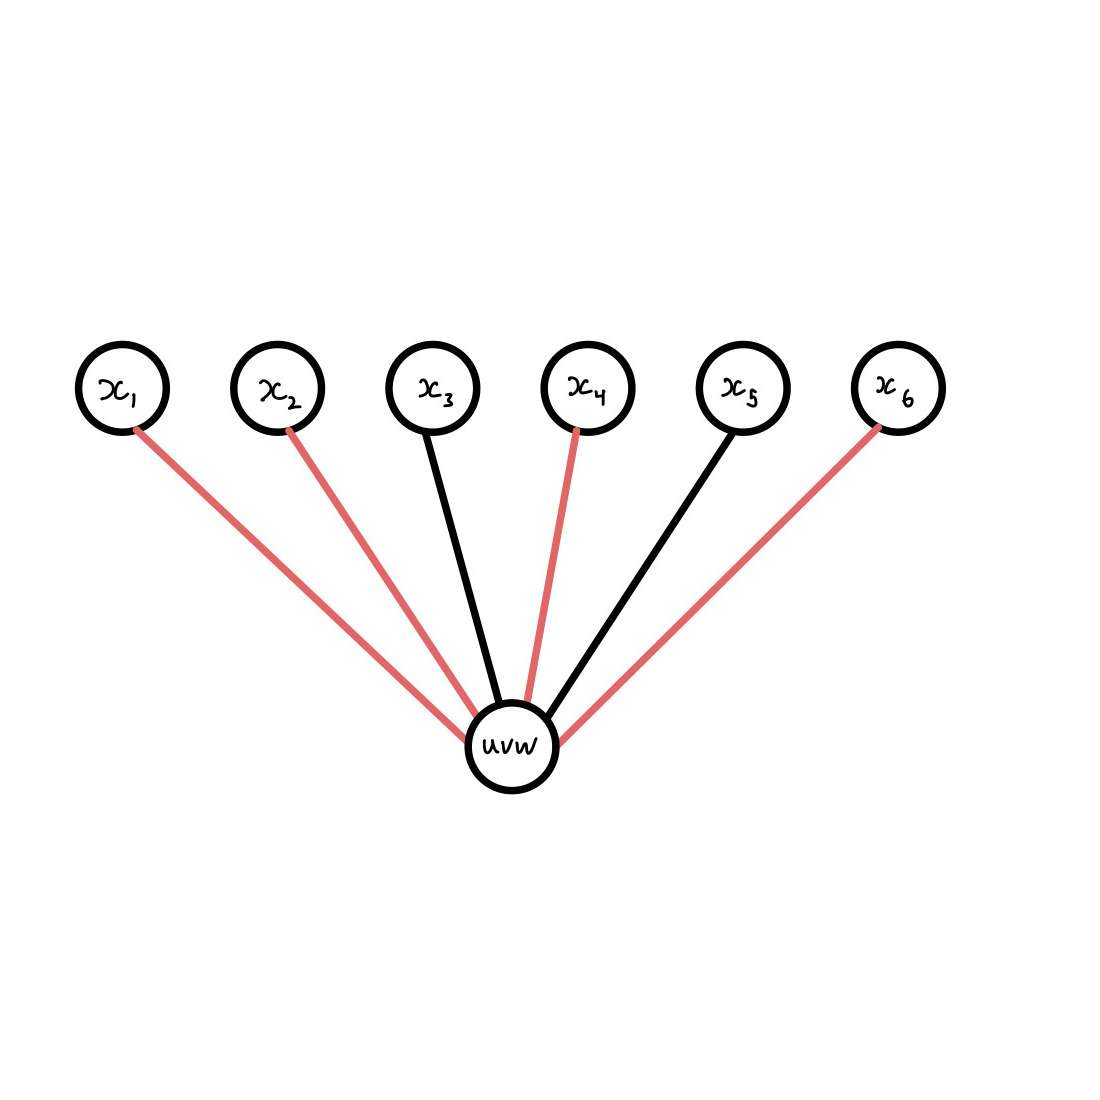
\includegraphics[width=0.5\textwidth]{images/cropped-12.jpg}
\end{frame}

\begin{frame}{Formal Definition of Contraction}
    Suppose we are contracting two nodes $u, v$ in $G$ into one node called $uv$. 
    
    \begin{itemize}
        \item For every neighbor $x$ of $u$ or $v$: \pause
        \begin{itemize}
            \item If $x$ is a black neighbor of both $u$ and $v$, then $x$ is now a black neighbor of $uv$
            \item Otherwise, $x$ is a red neighbor of $u$ and $v$
        \end{itemize} \pause
        \item All other edges are left alone and maintain their color
    \end{itemize}
\end{frame}

\begin{frame}{Twin-width}
    \begin{itemize}
        \item Repeatedly applying the contraction operation to nodes of $G$ produces a \textcolor{sigma@mainblue}{\emph{contraction sequence}} of graphs $G = G_n \to G_{n - 1} \to \cdots \to G_2 \to G_1 = K_1$ \pause
        \item The sequence is a \textcolor{sigma@mainblue}{\emph{$d$-sequence}} if the maximum number of red edges in any of the $G_i$ in the contraction sequence is $d$ \pause
        \item The \textcolor{sigma@mainblue}{\emph{twin-width}} of $G$ is the minimum $d$ such that there exists a $d$-sequence of $G$
    \end{itemize}
\end{frame}

\begin{frame}{Observations}
    \begin{itemize}
        \item The graph remains connected as we do this \pause
        \item This process will terminate (finitely many nodes and edges) \pause
        \item The number of red edges may increase or decrease
    \end{itemize}
\end{frame}

\begin{frame}{Why do We Care?}
    \begin{itemize}
        \item We can speed up certain algorithms \pause
        \item If we have the $d$-sequence for a graph, we can decompose the graph into complete bipartite graphs and do breadth-first-search in $O(n \log n)$ time \cite{Twin-width-III}
        \item This works even if the number of edges is $O\pqty{n^2}$
    \end{itemize}
\end{frame}

\section{Computing Twin-width}
\frame{\sectionpage}

\begin{frame}{It's Hard}
    \begin{itemize}
        \item There are very few practical algorithms for computing the twin-width of a graph in general \pause
        \item There are some things known for special cases
        \begin{itemize}
            \item Cographs are the graphs with twin-width zero 
            \item $d$-dimensional graphs have twin-width $\leq 3d$ \cite{Twin-width-I}
            \item Planar graphs have twin-width $\leq 9$, and bipartite planar graphs have twin-width $\leq 6$ \cite{planar}
            \item Graphs with 4 vertices have twin-width $\leq 1$ and graphs with 5 vertices have twin-width $\leq 2$ \cite{computation}
            \item In general, bipartite graphs may have arbitrarily large twin-width
        \end{itemize}
    \end{itemize}
\end{frame}

\begin{frame}{SAT Solvers}
    \begin{itemize}
        \item Given a boolean formula consisting of variables, \texttt{and} gates, and \texttt{or} gates, we want to find a satisfying assignment \pause
        \item This is a problem that appears in many places, so readily available \textcolor{sigma@mainblue}{\emph{SAT Solvers}} exist \pause
        \item \cite{SAT} found a way to encode twin-width into a SAT formula
        \item This is one of the only ways we can reasonable compute twin-widths
    \end{itemize}
\end{frame}

\section{PACE 2023}
\frame{\sectionpage}

\begin{frame}{A Programming Competition}
    \begin{itemize}
        \item \textbf{P}arameterized \textbf{A}lgorithms and \textbf{C}omputational \textbf{E}xperiments is a long-term programming competition
        \item Our goal will be to devise an efficient algorithm to compute the twin-width $d$ of arbitrary graphs and their $d$-sequence
        \begin{itemize}
            \item Exact Track: Compute the exact sequence
            \item Heuristic Track: Compute an approximate sequence 
        \end{itemize}
    \end{itemize}
\end{frame}

\begin{frame}{The Club Submission}
    \begin{itemize}
        \item I only found out about this recently so we are a bit behind
        \item We should make on submission on one track
        \begin{itemize}
            \item I was thinking about focusing on the exact track
        \end{itemize}
        \item There are 100 public test cases + 100 test cases
        \item Score = the number of test cases we can solve in a given time limit
        \item My goal is just to put together something and see how well we do
    \end{itemize}
\end{frame}

\font\eightss=cmssq8
\font\eightssi=cmssqi8
\newcommand\quoteAuthorDate[3]{\begingroup
  \baselineskip 10pt
  \parfillskip 0pt
  \interlinepenalty 10000 % not needed in example
  \leftskip 0pt plus 40pc minus \parindent
  \let\rm=\eightss
  \let\sl=\eightssi
  \everypar{\sl}#1\par
  \nobreak\smallskip
  \noindent\rm--- #2\unskip\enspace(#3)\par
  \endgroup}
% If someone can figure out how to horizontally center this and make the text bigger that'd be cool
% \begin{frame}
%     \begin{center}
%         \item \quoteAuthorDate{So long and thanks for all the fish!}{DOUGLAS ADAMS}{\color{sigma@mainblue} 1979}
%     \end{center}
% \end{frame}

% Remove this slide if you came up with all the material yourself
\begin{frame}{Bibliography}
    {\tiny \bibliography{refs}}
    \bibliographystyle{alpha}
\end{frame}

\end{document}